\documentclass[12pt, letterpaper]{article}

\usepackage{hyperref} % para manejar hipervinculos
\usepackage[spanish]{babel} % Para palabras en espanhol
\usepackage{graphicx} % LaTeX package to import graphics
\graphicspath{{../images/}} % configuring the graphicx package
\usepackage[spanish]{babel} % para que LaTeX corte palabras
\usepackage[dvipsnames]{xcolor} % color en el texto
\usepackage[backend=biber,style=numeric]{biblatex} % para la bibliografia.
\addbibresource{bibliografia.bib} % incluir el .bib
\hypersetup{ % configuracion de los hiper vinculos
    colorlinks=true,
    linkcolor=black,
    filecolor=black,      
    urlcolor=blue,
    citecolor=black, 
    pdftitle={Entrega5},
    pdfpagemode=FullScreen,
}
\usepackage{csquotes} % para que los textos citados esten con tipografia de acuerdo con las reglas de csquotes
\setcounter{biburlnumpenalty}{9000} % Para el line breaker en URL con numeros (que tambien afecta a la bibliografia)
\setcounter{biburllcpenalty}{9000} % Para el line breaker en URL con letras minuculas (que tambien afecta a la bibliografia)
\setcounter{biburlucpenalty}{9000} % Para el line breaker en URL con letras mayusculas (que tambien afecta a la bibliografia)

\begin{document}
% Portada
\begin{titlepage}
  \begin{center}
      \Large{Universidad Catolica "Nuestra señora de la Asuncion" \\
      Facultad de ciencias y tecnologia \\
      Complementos de Informatica}
      
\includegraphics[width=0.8\textwidth]{UcaLogo.jpg}
      \LARGE{\textbf{Modelo predictivo para detectar la insuficiencia cardiaca
      }} \\
      \Large{Entrega 5 - Data mining}
      \vspace{1cm}
  \end{center}
      \large
      \textbf{Alumno: }Alain Vega \\
      \textbf{Profesor: }Wilfrido Felix Inchaustti Martínez
      \vfill
      \hfill{27 de Noviembre del 2023}
\end{titlepage}


\newpage
\tableofcontents % indice
\newpage

% Contenidos
\section{Comprension del negocio}
Las enfermedades cardiovasculares (ECV) son la principal causa de muerte a nivel mundial, 
cobrando la vida de aproximadamente 17.9 millones de personas cada año, 
lo que representa el 31\% de todas las muertes en todo el mundo. 
Cuatro de cada 5 muertes por ECV son causadas por ataques cardíacos y accidentes cerebrovasculares, 
y un tercio de estas muertes ocurren prematuramente en personas menores de 70 años. 

La insuficiencia cardíaca es un evento común causado por las ECV.
Las personas con enfermedades cardiovasculares o que tienen un alto riesgo cardiovascular 
(debido a la presencia de uno o más factores de riesgo como hipertensión, diabetes, 
hiperlipidemia o enfermedades ya establecidas) necesitan una detección temprana y gestión, 
en la cual un modelo de aprendizaje automático puede ser de gran ayuda. 
\cite*{dataset}

\section{Comprension de los datos}
\subsection{Conjunto de datos}
Los datos a utilizar en el proyecto sera un archivo .csv 
(\textit{Comma Separated Values}) llamado \textit{heart.csv} 
que se obtuvo de la plataforma web \textit{Kaggle} \cite{dataset}
el cual de inicio contiene 12 columnas, las cuales son:
\begin{enumerate}
    \item{\textbf{\textit{Age}}. edad del paciente} 
    \item{\textbf{\textit{Sex}}. sexo del paciente, donde:
    \begin{itemize}
        \item{\textbf{M}}: Masculino
        \item{\textbf{F}}: Femenino
    \end{itemize}
    }
    \item{\textbf{\textit{ChestPain}}. tipo de dolor en el pecho, el cual puede ser: 
    \begin{itemize}
        \item{\textbf{TA}}: \textit{Typical Angina}, es decir angina tipica
        \item{\textbf{ATA}}: \textit{Atypical Angina}
        \item{\textbf{NAP}}: \textit{Non-Anginal Pain}
        \item{\textbf{ASY}}: \textit{Asymptomatic}
    \end{itemize}
    La angina de pecho es un tipo de dolor de pecho causado por la reduccion del flujo
    salguineo al corazon. El dolor a menudo se describe como un dolor constrictivo, 
    presión, pesadez, opresión o dolor en el pecho. El paciente siente como si tuviera
    un gran peso apoyado en el pecho. \cite{angina}
    }
    \item{\textbf{\textit{RestingBP}}. presión arterial en reposo (sistólica)
    medido en mililitros de mercurio [mmHg]
    
    La presión arterial es una medida de la fuerza que utiliza el corazón para bombear
    sangre por el cuerpo. Se mide en milímetros de mercurio [mmHg] y se expresa en 2 cifras:
    \begin{itemize}
        \item{presión sistólica: la presión cuando el corazón expulsa la sangre}
        \item{presión diastólica: la presión cuando el corazón descansa entre latidos}
    \end{itemize}
    Por ejemplo, una presión arterial de \textquotedblleft{}140 sobre 90\textquotedblright{}
    o 140/90 mmHg, significa una presión sistólica de 140 mmHg y una presión diastólica
    de 90 mmHg. \cite{presion-arterial}
    }
    \item{\textbf{\textit{Cholesterol}}. Colesterol serico 
    medido en miligramos por decilitro de sangre [mm/dl]
    
    El colesterol es una sustancia grasa (un lípido) presente en todas las células del organismo.
    Los niveles de colesterol en sangre, que indican la cantidad de lípidos o grasas presentes
    en la sangre, se expresan en miligramos por decilitro [mg/dl]
    La sangre lleva el colesterol a las células en partículas transportadoras especiales 
    denominadas «lipoproteínas». Dos de las lipoproteínas más importantes son:
    \begin{itemize}
        \item{lipoproteína de baja densidad (LDL) - tambien conocida como colesterol malo}
        \item{lipoproteína de alta densidad (HDL) - tambien conocida como colesterol malo}
    \end{itemize}

    El colesterol total (serico) en sangre es la suma del colesterol transportado en las 
    partículas de LDL, HDL y otras lipoproteínas. \cite{colesterol}
    }
    \item{\textbf{\textit{FastingBS}}. azúcar en sangre (glucosa) en ayunas
    medido en miligramos por decilitro [mg/dl], puede ser:
    \begin{itemize}
        \item{1: Si \textit{FastingBS} \(>\) 120 [mg/dl]}
        \item{0: Caso contrario}
    \end{itemize}
    }
    \item{\textbf{\textit{RestingECG}}. resultados del electrocardiograma 
    en reposo, puede ser:
    \begin{itemize}
        \item{\textbf{Normal}: normal
        
        Indica que no se observaron anormalidades significativas en el electrocardiograma. 
        Las ondas y complejos están dentro de los rangos normales.
        }
        \item{\textbf{ST}: tener anomalía de la onda ST-T 
        (inversiones de la onda T y/o elevación o depresión del ST \(>\) 0,05 mV)

        % Con la figura \ref{fig:ST}, 
        El segmento ST es la sección plana e isoeléctrica 
        del ECG entre el final de la onda S (el punto J) y el comienzo de la onda T.
        El segmento ST representa el intervalo entre la despolarización y la repolarización 
        ventricular. \cite{ST}

        \begin{figure}
            \centering
            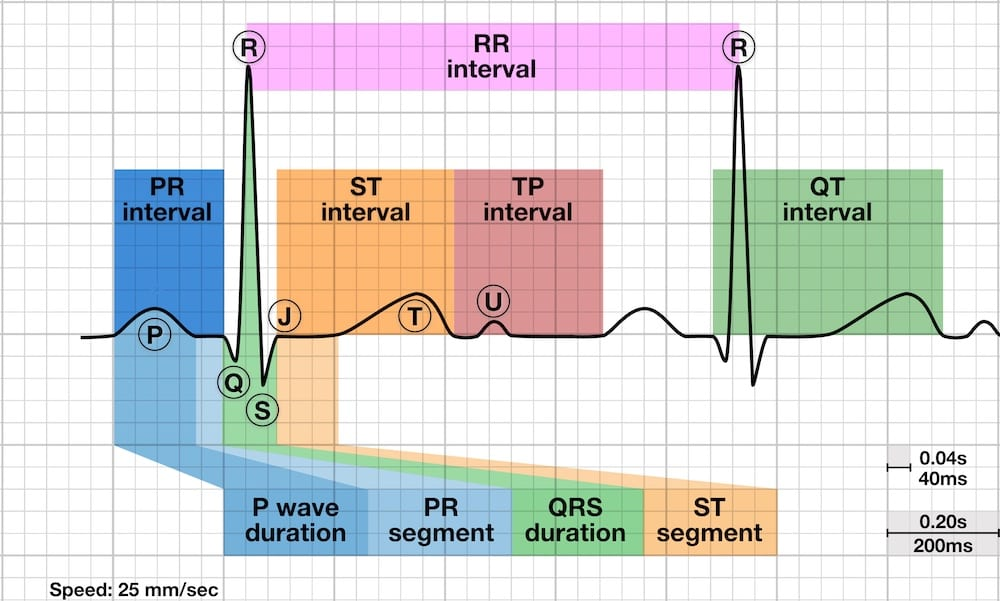
\includegraphics[scale=0.38]{ST_image.jpg}
            \caption{ECG de un corazon \cite{ST}}
            \label{fig:ST}
        \end{figure}

        }
        \item{\textbf{LVH}: muestra probable o definitiva hipertrofia ventricular 
        izquierda según los criterios de Estes
       
        Se refiere a un aumento en el tamaño de las fibras miocárdicas en la cámara de bombeo 
        cardíaca principal.
        Esto sugiere un agrandamiento anormal del músculo del ventrículo izquierdo del corazón.
        \cite{LVH}
        }
    \end{itemize}

    Un ECG de diagnóstico en reposo (electrocardiograma) registra la actividad eléctrica 
    del corazón mientras está en reposo. Proporciona información sobre su frecuencia y 
    ritmo cardíaco y también puede mostrar si hay agrandamiento del corazón o 
    evidencia de un ataque cardíaco previo. \cite{electrocardiograma}
    } 
    \item{\textbf{\textit{MaxHR}}. frecuencia cardíaca máxima alcanzada
    medido en pulsaciones por minuto [ppm]}
    \item{\textbf{\textit{ExerciseAngina}}. angina inducida por el ejercicio, puede ser:
    \begin{itemize}
        \item{\textbf{Y}}: Si
        \item{\textbf{N}}: No
    \end{itemize}
    }
    \item{\textbf{\textit{OldPeak}}. pico antiguo = ST [Valor numérico medido en depresión]}
    \item{\textbf{\textit{ST\_Slope}}. pendiente del segmento ST 
    durante un ejercicio físico máximo en una prueba de 
    esfuerzo cardíaco. Puede ser:
    \begin{itemize}
        \item{\textbf{Up}}: ascendente
        \item{\textbf{Flat}}: plano
        \item{\textbf{Down}}: descendente
    \end{itemize}
    }
    \item{\textbf{\textit{HeartDisease}}. sufrio de insuficiencia cardiaca
    \begin{itemize}
        \item{\textbf{1}}: insuficiencia cardiaca
        \item{\textbf{0}}: normal
    \end{itemize}
    }
\end{enumerate}
El \textit{dataset} dispone de 918 muestras en total para ser analizadas.

\subsection{Missing values}
Un valor faltante puede significar varias cosas diferentes. 
Quizás el campo no era aplicable, el evento no ocurrió o los datos no estaban disponibles. 
Podría ser que la persona que ingresó los datos no conocía el valor correcto o no le importaba 
si un campo no estaba completado. \cite{missin_values}

El \textit{dataset} no posee valores faltantes en ningun registro, como lo muestra la figura
\ref{fig:missing_values}
\begin{figure}
    \centering
    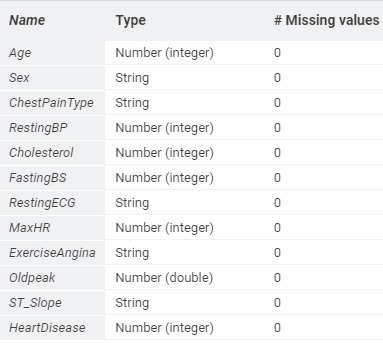
\includegraphics[scale=1]{missing_values.jpg}
    \caption{Missing values en el dataset heart.csv}
    \label{fig:missing_values}
\end{figure}
\newpage
\subsection{Ruidos y anomalias}

Un ruido es un dato o un conjunto de datos que agregan informacion sin sentido a la muestra.
\cite{ruido}

Un valor atípico o dato anomali (\textit{outlier}, en inglés) 
es una observación que numéricamente es muy distinta al resto de elementos de una muestra.
\cite{anomalia}

\subsubsection{Ruidos}
En la columna \textit{RestingBP} se encontro un registro cuyo valor es 0, cosa que es imposible.
Se puede apreciar en la figura \ref{fig:presion-arterial}

\begin{figure}
    \centering
    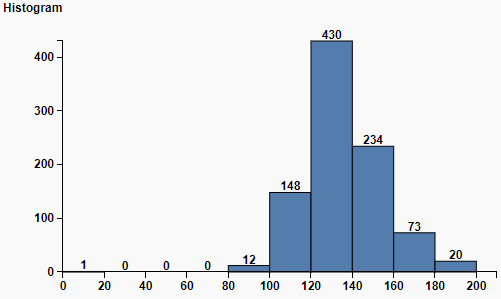
\includegraphics[scale=1]{RestingBP.png}
    \caption{Histograma de la presion arterial}
    \label{fig:presion-arterial}
\end{figure}


En la columna \textit{Cholesterol} se encontraron una cantidad de 172 registros cuyos valores 
son 0, cosa que es imposible. Se puede apreciar en la figura \ref{fig:colesterol}

\begin{figure}
    \centering
    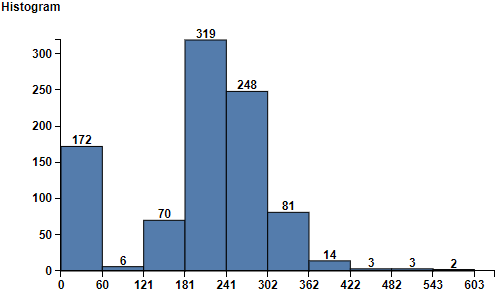
\includegraphics[scale=1]{Cholesterol.png}
    \caption{Histograma del colesterol}
    \label{fig:colesterol}
\end{figure}


\subsubsection{Anomalias}
En la columna \textit{Cholesterol} se encontraron 8 registros cuyos valores son mayores a 420,
donde se los considera anomalias. Se puede apreciar en la figura \ref{fig:colesterol}

\subsection{Redundancia}
La redundancia a nivel de datos en un conjunto de datos hace referencia a que 2 o mas datos
presentan la misma informacion.

Durante la exploracion no se encontraron valores o campos redundantes
misma informacion, esto se visualizara mejor a continuacion.
\subsubsection{Correlacion}
La correlación mide la fuerza de la relación entre dos variables. 
Proporciona una idea de cómo se relacionan las variables y cómo se afectan entre sí. 
\cite{correlacion}

\begin{figure}
    \centering
    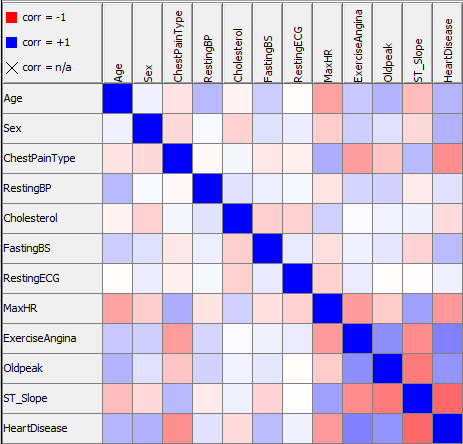
\includegraphics[scale=1]{correlacion.png}
    \caption{Matriz de correlacion en el dataset heart.csv}
    \label{fig:correlacion}
\end{figure}

Las correlaciones de datos se pueden visualizar en la figura \ref{fig:correlacion}.


La correlacion mas fuerte en el conjunto de datos se da entre las 
columnas: \textit{heartDisease, ST\_Slope} con valor de -59.19\%.
Como el maximo valor no llega siquiera al 60\% se deduce que no se disponen de datos redundantes.


\section{Preparacion de los datos}
El dataset, asi como se expuso en la fase 2, no presenta muchas dificultades en cuanto a la
calidad de los datos, esto resalta su confiabilidad para la construccion posterior de un
modelo que ayude a la deteccion de posibles insuficiencias cardiacas.

\subsection{Tratamiento de missing values}
Un valor faltante puede significar varias cosas diferentes. 
Quizás el campo no era aplicable, el evento no ocurrió o los datos no estaban disponibles. 
Podría ser que la persona que ingresó los datos no conocía el valor correcto o no le importaba 
si un campo no estaba completado. \cite{missin_values}

Como se expuso en el documento de la entrega 2, en el \textit{dataset heart.csv}
no se encuentran \textit{missing values} por lo cual el tratamiento es no hacer nada.

\subsection{Tratamiento de ruidos}
Un ruido es un dato o un conjunto de datos que agregan informacion sin sentido a la muestra.
\cite{ruido}

En las columnas \textit{RestingBP} y \textit{Cholesterol} se detectaron ruidos. 
La estrategia empleada de abordaje consiste en reemplazar los registros ruidosos
con el promedio de valores libre de ruido.

\subsection{Tratamiento de anomalias}
Un valor atípico o dato anomali (\textit{outlier}, en inglés) 
es una observación que numéricamente es muy distinta al resto de elementos de una muestra.
\cite{anomalia}

En la columna \textit{Cholesterol} se detectaron anomalias, como se expuso en la entrega 2. 
La estrategia empleada de abordaje consiste en reemplazar los registros anomalos
con el promedio de valores libre de anomalias.

\begin{figure}
    \centering
    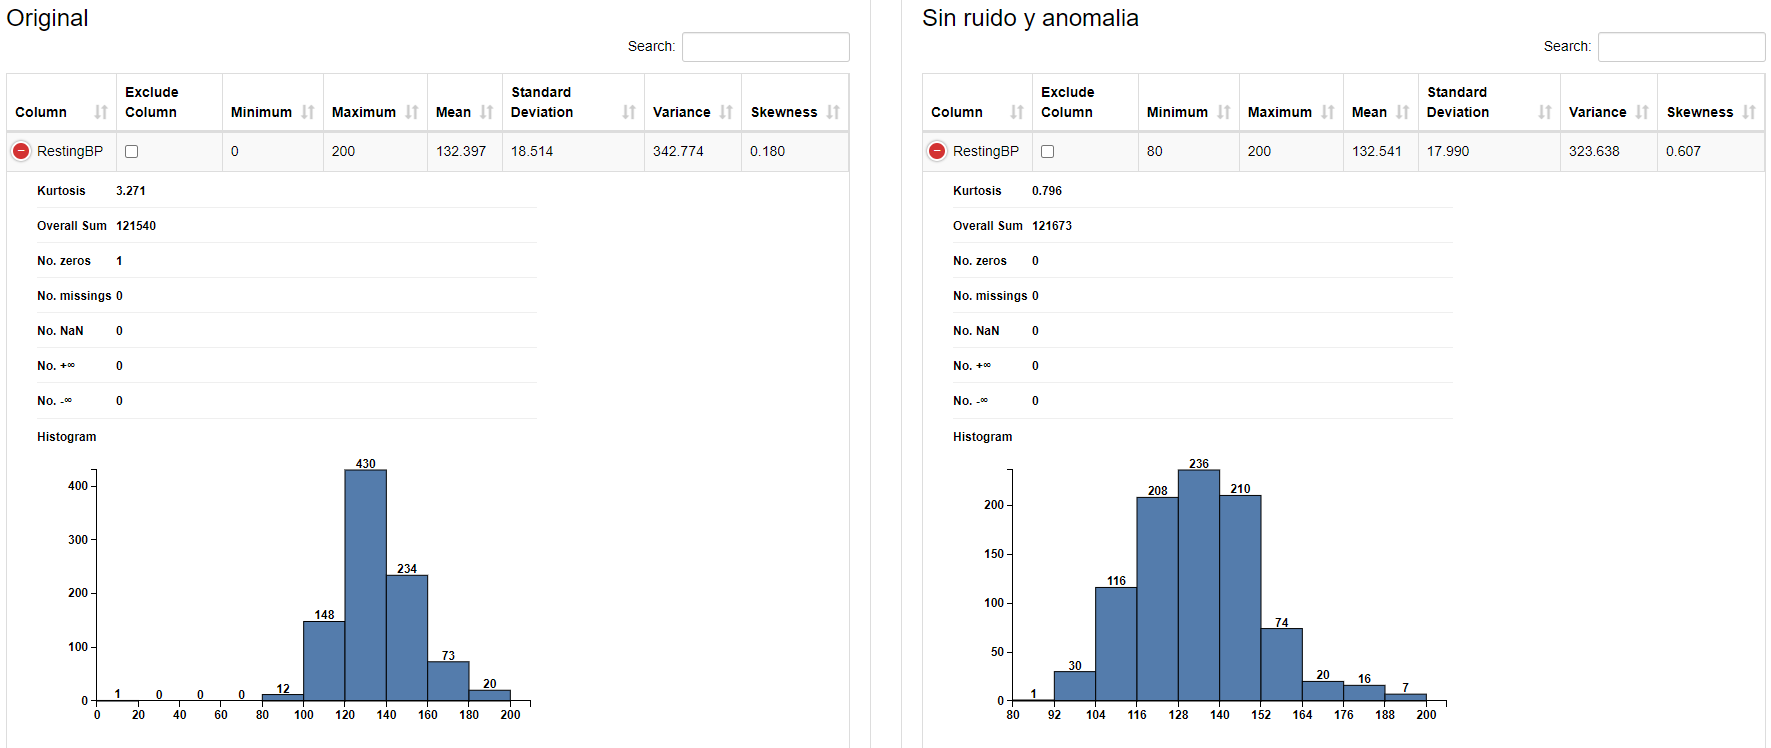
\includegraphics[scale=0.29]{comparativa-RestingBP.png}
    \caption{Comparativa de la distribucion del RestingBP (presion arterial), antes 
    despues del tratamiento de rudios y anomalias}
    \label{fig:comparativa-RestingBP}
\end{figure}

\begin{figure}
    \centering
    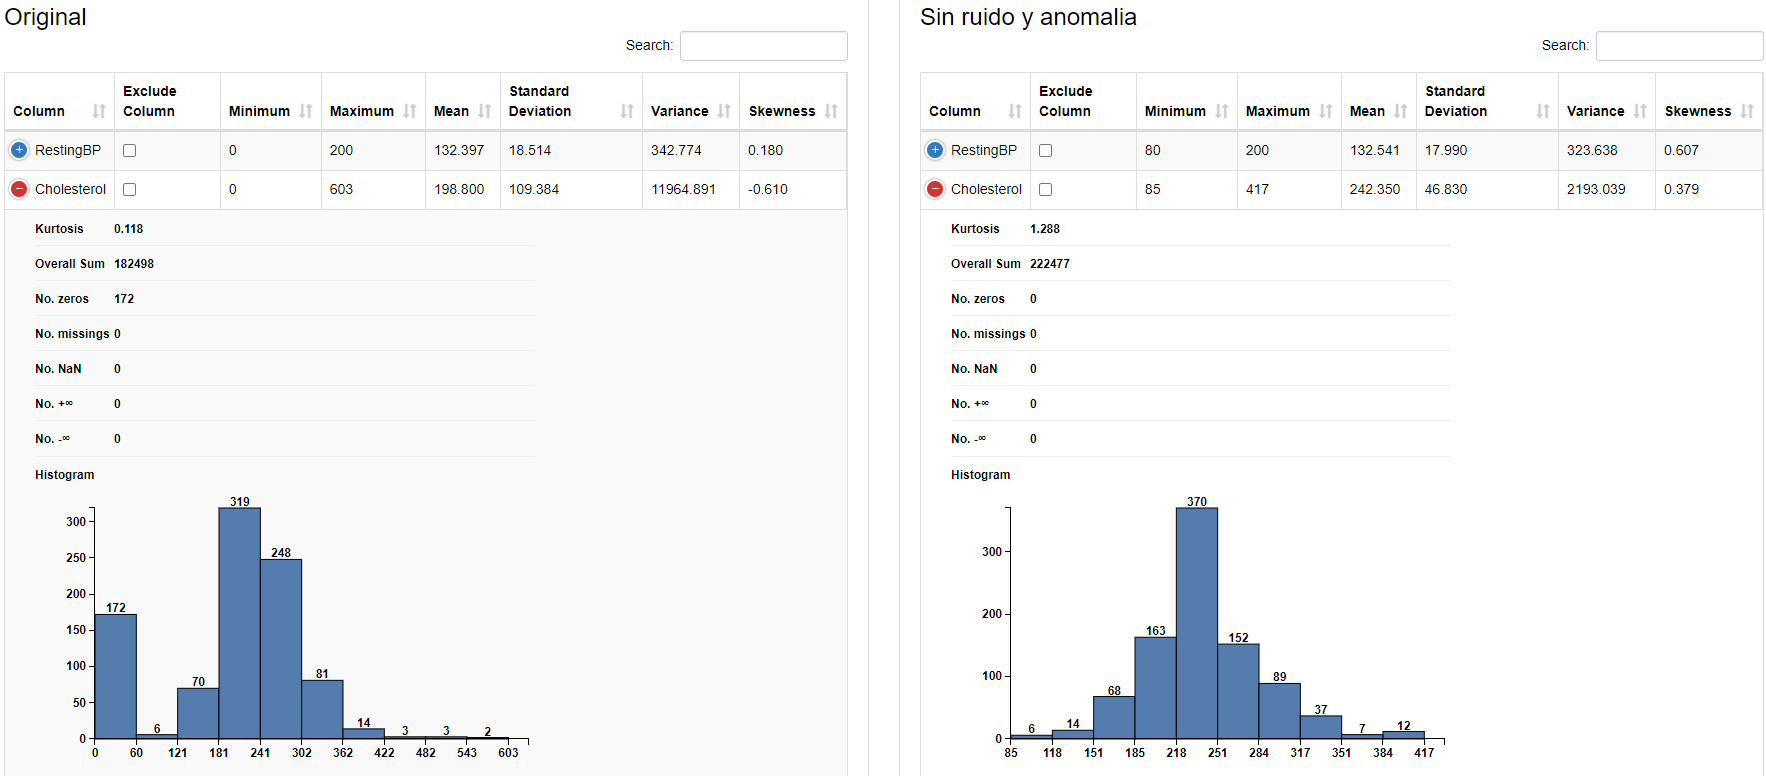
\includegraphics[scale=0.29]{comparativa-Cholesterol.png}
    \caption{Comparativa de la distribucion del Cholesterol, antes 
    despues del tratamiento de rudios y anomalias}
    \label{fig:comparativa-Cholesterol}
\end{figure}

\subsection{Manejo de variables categoricas}
Las columnas \textit{Sex}, \textit{ChestPain}, \textit{RestingECG}, \textit{ExerciseAngina} y
\textit{ST\_Slope} eran de tipo string que correspondian a diferentes categorias de cada
correspondiente concepto. 

\subsection{Normalizacion}
No se aplico ninguna normalizacion al \textit{dataset} debido a la buena calidad del
conjunto de datos.

\subsection{Diccionario de datos finales a utilizar}
Luego de la preparacion de los datos, se obtiene el .csv final
(\textit{Comma Separated Values}) el cual cuenta con 12 columnas, las cuales:
\begin{enumerate}
    \item{\textbf{\textit{Age}}. edad del paciente} 
    \item{\textbf{\textit{Sex}}. sexo del paciente, donde:
    \begin{itemize}
        \item{\textbf{0}}: Masculino
        \item{\textbf{1}}: Femenino
    \end{itemize}
    }
    \item{\textbf{\textit{ChestPain}}. tipo de dolor en el pecho, el cual puede ser: 
    \begin{itemize}
        \item{\textbf{0}}: \textit{Typical Angina}, es decir angina tipica
        \item{\textbf{1}}: \textit{Atypical Angina}
        \item{\textbf{2}}: \textit{Non-Anginal Pain}
        \item{\textbf{3}}: \textit{Asymptomatic}
    \end{itemize}
    La angina de pecho es un tipo de dolor de pecho causado por la reduccion del flujo
    salguineo al corazon. El dolor a menudo se describe como un dolor constrictivo, 
    presión, pesadez, opresión o dolor en el pecho. El paciente siente como si tuviera
    un gran peso apoyado en el pecho. \cite{angina}
    }
    \item{\textbf{\textit{RestingBP}}. presión arterial en reposo (sistólica)
    medido en mililitros de mercurio [mmHg]
    
    La presión arterial es una medida de la fuerza que utiliza el corazón para bombear
    sangre por el cuerpo. Se mide en milímetros de mercurio [mmHg] y se expresa en 2 cifras:
    \begin{itemize}
        \item{presión sistólica: la presión cuando el corazón expulsa la sangre}
        \item{presión diastólica: la presión cuando el corazón descansa entre latidos}
    \end{itemize}
    Por ejemplo, una presión arterial de \textquotedblleft{}140 sobre 90\textquotedblright{}
    o 140/90 mmHg, significa una presión sistólica de 140 mmHg y una presión diastólica
    de 90 mmHg. \cite{presion-arterial}
    }
    \item{\textbf{\textit{Cholesterol}}. Colesterol serico 
    medido en miligramos por decilitro de sangre [mm/dl]
    
    El colesterol es una sustancia grasa (un lípido) presente en todas las células del organismo.
    Los niveles de colesterol en sangre, que indican la cantidad de lípidos o grasas presentes
    en la sangre, se expresan en miligramos por decilitro [mg/dl]
    La sangre lleva el colesterol a las células en partículas transportadoras especiales 
    denominadas «lipoproteínas». Dos de las lipoproteínas más importantes son:
    \begin{itemize}
        \item{lipoproteína de baja densidad (LDL) - tambien conocida como colesterol malo}
        \item{lipoproteína de alta densidad (HDL) - tambien conocida como colesterol malo}
    \end{itemize}

    El colesterol total (serico) en sangre es la suma del colesterol transportado en las 
    partículas de LDL, HDL y otras lipoproteínas. \cite{colesterol}
    }
    \item{\textbf{\textit{FastingBS}}. azúcar en sangre (glucosa) en ayunas
    medido en miligramos por decilitro [mg/dl], puede ser:
    \begin{itemize}
        \item{1: Si \textit{FastingBS} \(>\) 120 [mg/dl]}
        \item{0: Caso contrario}
    \end{itemize}
    }
    \item{\textbf{\textit{RestingECG}}. resultados del electrocardiograma 
    en reposo, puede ser:
    \begin{itemize}
        \item{\textbf{0}: normal
        
        Indica que no se observaron anormalidades significativas en el electrocardiograma. 
        Las ondas y complejos están dentro de los rangos normales.
        }
        \item{\textbf{1}: tener anomalía de la onda ST-T 
        (inversiones de la onda T y/o elevación o depresión del ST \(>\) 0,05 mV)

        % Con la figura \ref{fig:ST}, 
        El segmento ST es la sección plana e isoeléctrica 
        del ECG entre el final de la onda S (el punto J) y el comienzo de la onda T.
        El segmento ST representa el intervalo entre la despolarización y la repolarización 
        ventricular. \cite{ST}

        }
        \item{\textbf{2}: muestra probable o definitiva hipertrofia ventricular 
        izquierda según los criterios de Estes
       
        Se refiere a un aumento en el tamaño de las fibras miocárdicas en la cámara de bombeo 
        cardíaca principal.
        Esto sugiere un agrandamiento anormal del músculo del ventrículo izquierdo del corazón.
        \cite{LVH}
        }
    \end{itemize}

    Un ECG de diagnóstico en reposo (electrocardiograma) registra la actividad eléctrica 
    del corazón mientras está en reposo. Proporciona información sobre su frecuencia y 
    ritmo cardíaco y también puede mostrar si hay agrandamiento del corazón o 
    evidencia de un ataque cardíaco previo. \cite{electrocardiograma}
    } 
    \item{\textbf{\textit{MaxHR}}. frecuencia cardíaca máxima alcanzada
    medido en pulsaciones por minuto [ppm]}
    \item{\textbf{\textit{ExerciseAngina}}. angina inducida por el ejercicio, puede ser:
    \begin{itemize}
        \item{\textbf{1}}: Si
        \item{\textbf{0}}: No
    \end{itemize}
    }
    \item{\textbf{\textit{OldPeak}}. pico antiguo = ST [Valor numérico medido en depresión]}
    \item{\textbf{\textit{ST\_Slope}}. pendiente del segmento ST 
    durante un ejercicio físico máximo en una prueba de 
    esfuerzo cardíaco. Puede ser:
    \begin{itemize}
        \item{\textbf{1}}: ascendente
        \item{\textbf{0}}: plano
        \item{\textbf{-1}}: descendente
    \end{itemize}
    }
    \item{\textbf{\textit{HeartDisease}}. sufrio de insuficiencia cardiaca
    \begin{itemize}
        \item{\textbf{si}}: insuficiencia cardiaca
        \item{\textbf{no}}: normal
    \end{itemize}
    }
\end{enumerate}
El \textit{dataset} dispone de 918 muestras en total para ser analizadas.
La figura \ref{fig:Workflow3} muestra el workflow correspondiente.

\begin{figure}
    \centering
    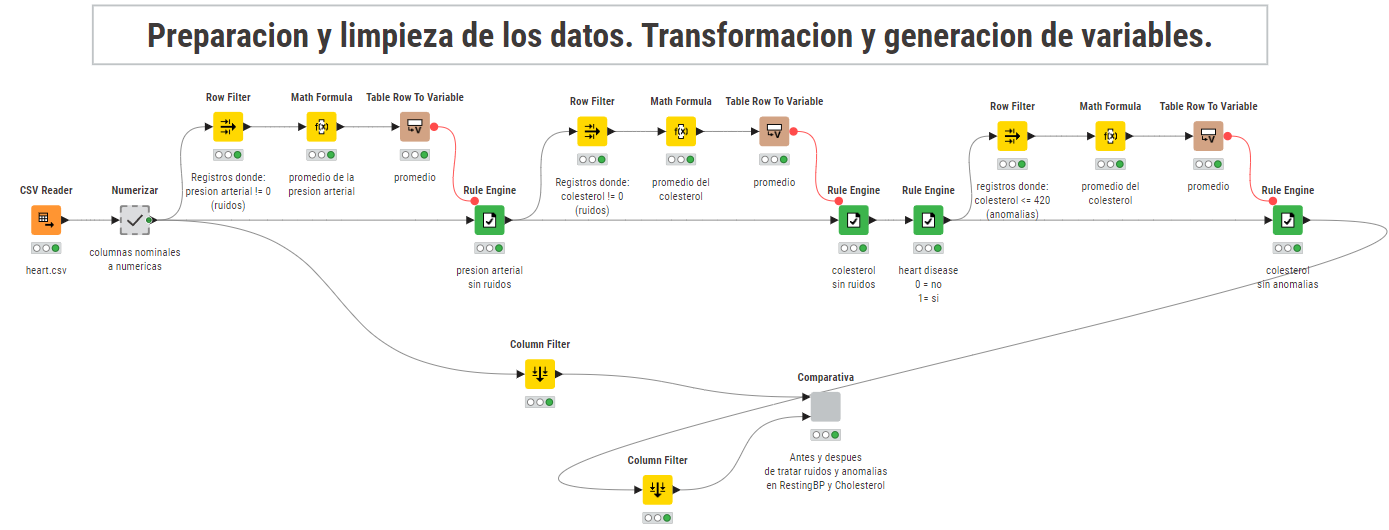
\includegraphics[scale=0.37]{entrega3.png}
    \caption{Workflow de la prepacacion y limpieza de datos, en knime.}
    \label{fig:Workflow3}
\end{figure}

\section{Modelado y evaluacion}
Para la construccion del modelo vamos a utilizar el conjunto de datos ya procesados en la 
etapa previa. 
Con motivo de mejorar la confiabilidad del modelo, vamos a implementar varias tecnicas para 
cumplir con nuestra tarea: predecir cuando una persona puede sufrir o no de 
insuficiencia cardiaca. 

Para lo cual, la siguiente tecnica de validacion fue elegida: \textbf{Cross validation}
con 5 particiones del conjunto de datos (\textit{folds}). 
Ya que el conjunto de pruebas de la validacion cruzada es significativamente mayor a que 
simplemente realizar un tipico \textit{train/test split} con 70\% pruebas - 30\% validacion. 
Se compararon las siguientes tecnicas:
\begin{itemize}
    \item{\textbf{Decision tree} gain ratio, no prunning, binario} 
    \item{\textbf{Logistic regression} minimos cuadrados, } 
    \item{\textbf{Random forest} gain ratio, 100 modelos, tamaño minimo del nodo = 3} 
    \item{\textbf{Gradient boosting (trees)} 200 modelos, profundidad del arbol = 4} 
    \item{\textbf{Naive bayes} probabilidad por defecto = 0,0001, desviacion estandar minima = 0,0001
    umbral desviacion estandar = 0} 
    \item{\textbf{Fuzzy logic} usar clase con mayor cobertura} 
    \item{\textbf{Neural network} 2 capas ocultas con 11 nodos cada una, 100 iteraciones} 
    \item{\textbf{Support vector machine (SVM)} kernel polinomial con valores por defecto} 
    \item{\textbf{K nearest neighbor} vecinos a partir de 3}
\end{itemize}
las figuras \ref{fig:tecnicas1}, \ref{fig:tecnicas2} y \ref{fig:tecnicas3} muestran la comparativa
entre estas tecnicas utilizando la validacion cruzada.

\begin{figure}
    \centering
    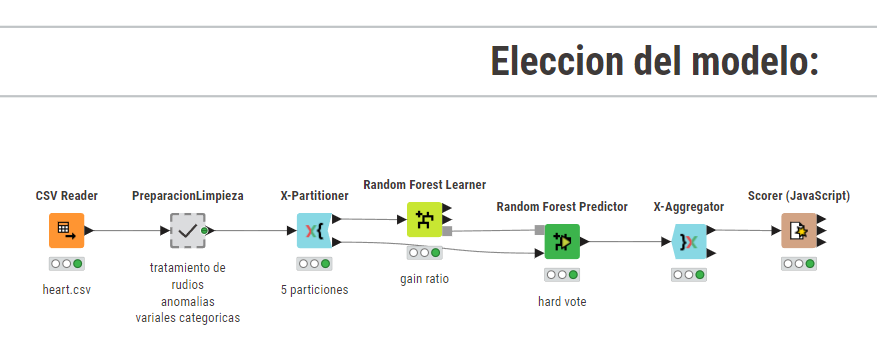
\includegraphics[scale=0.59]{entrega4.png}
    \caption{Workflow del modelado final, en knime.}
    \label{fig:Workflow4}
\end{figure}

\begin{figure}
    \centering
    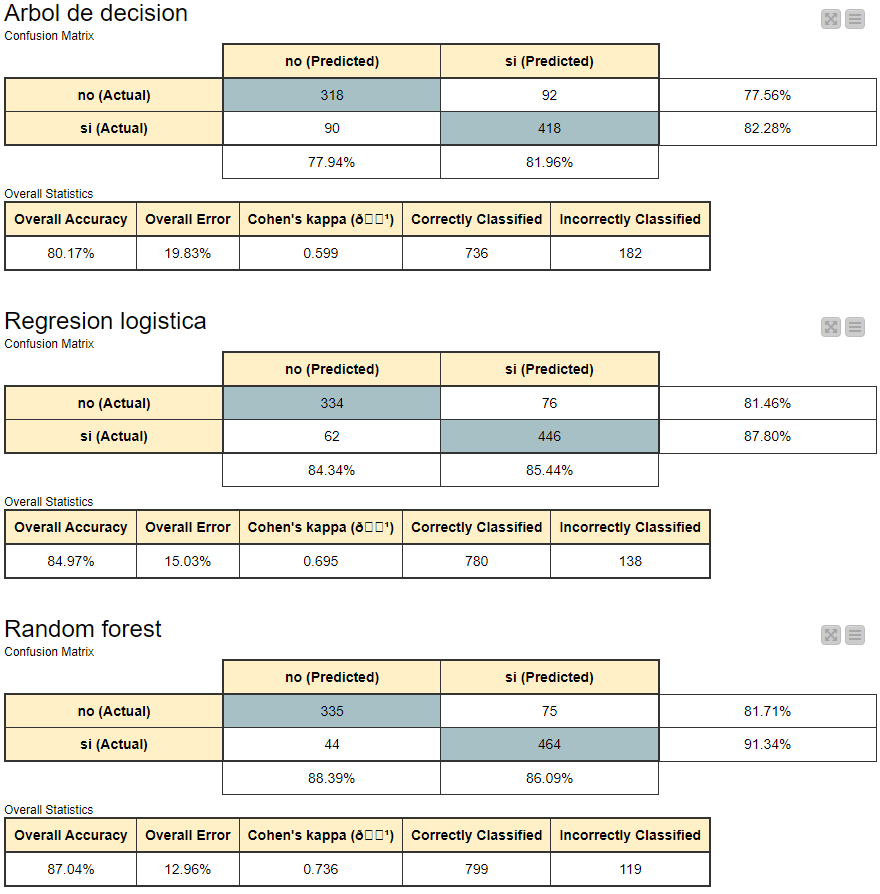
\includegraphics[scale=0.58]{tecnicas1.png}
    \caption{Evaluacion de estadisticas de diferentes tecnicas, parte 1}
    \label{fig:tecnicas1}
\end{figure}

\begin{figure}
    \centering
    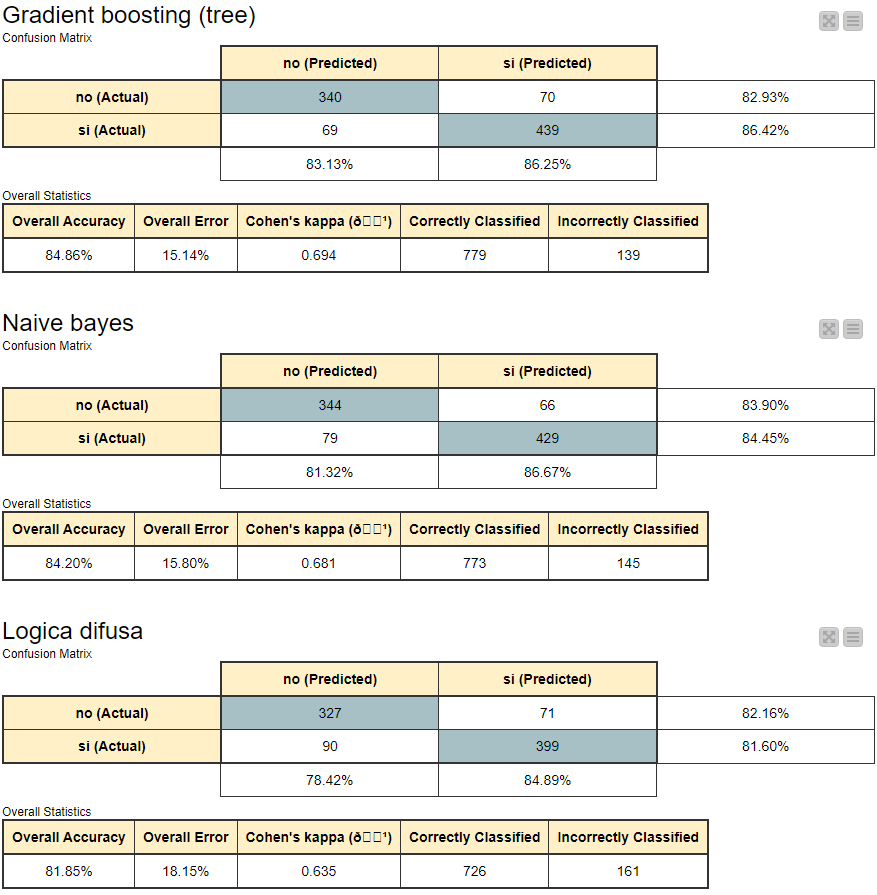
\includegraphics[scale=0.58]{tecnicas2.png}
    \caption{Evaluacion de estadisticas de diferentes tecnicas, parte 2}
    \label{fig:tecnicas2}
\end{figure}

\begin{figure}
    \centering
    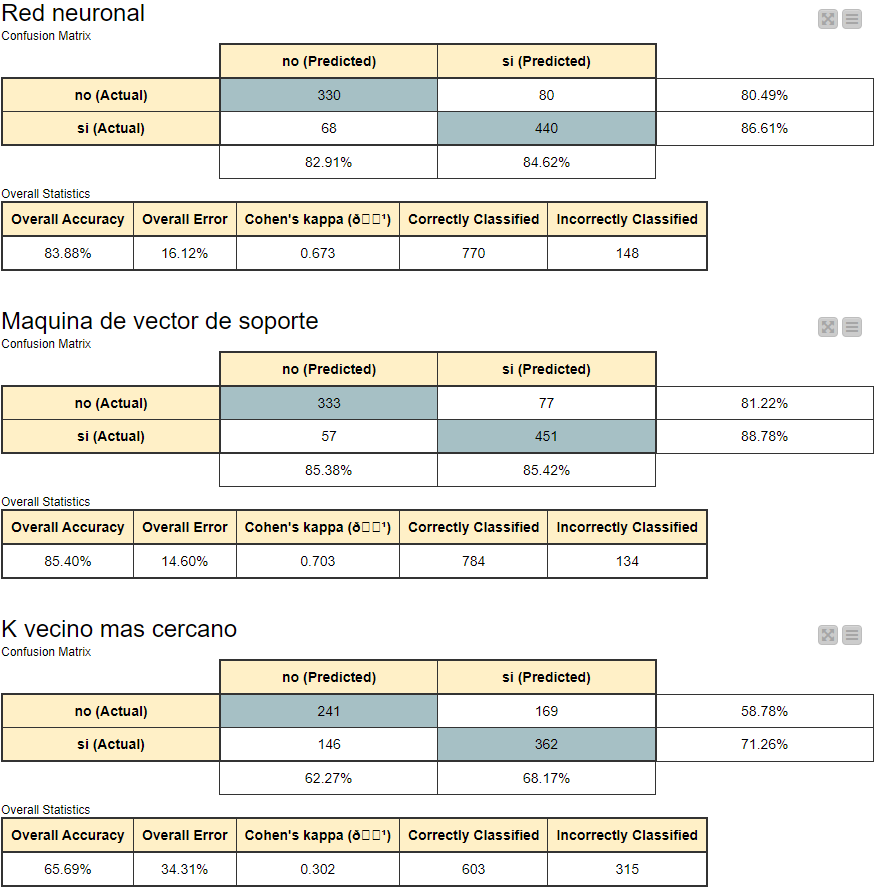
\includegraphics[scale=0.58]{tecnicas3.png}
    \caption{Evaluacion de estadisticas de diferentes tecnicas, parte 3}
    \label{fig:tecnicas3}
\end{figure}

La tecnica elegia fue el \textbf{Random forest} ya que obtiene mejores estadisticas en general 
en la serie de pruebas que se ejecutaron. Tambien y mas imporante, es la tenica que 
minimiza los falsos negativos, para este particular problema un falso negativo puede costar vidas.

Por lo tanto una vista simplificada del workflow lo muestra la figura \ref{fig:Workflow4}

Y por ultimo, una vista del workflow final, lo muestra la figura

\section{Implantacion}
Aunque el modelo ha demostrado ser prometedor en la predicción de la insuficiencia cardiaca, 
se reconoce la necesidad de una validación continua con mas datos, antes de su implantacion, 
ya que como se menciono al principio del documento, la muestra es de 918 personas. 

\newpage
\printbibliography

\end{document}